\section*{Question 5}
\textit{Calculate the autocorrelation function for both datasets. Compare the two curves and comment on the results.}

\begin{figure}[!ht]
\centering
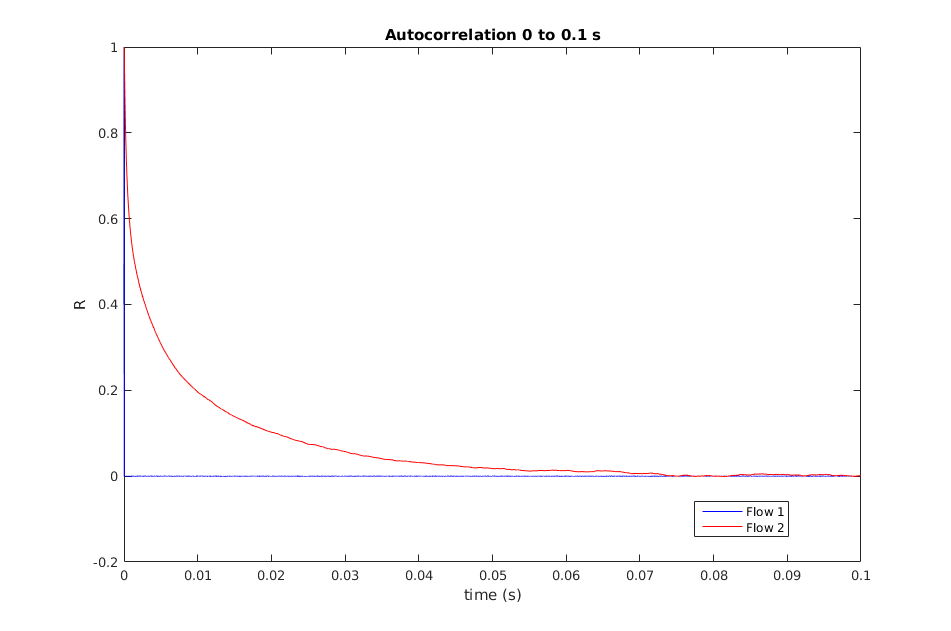
\includegraphics[scale=0.5]{./TEXT/auto1.png}
\caption{The comparison between the autocorrelation behaviours of the two flows from the origin to $0.1$ s.}
\label{auto1}
\end{figure}
Figure \ref{auto1} shows how sharply autocorrelation drops for the first flow case and in figure \ref{auto2} it can be seen how it oscilates around $0$, which is most probably the result of some signal or floating point operation error than an actual description of a phyisical property. Autocorrelation is also small for the second flow case but more pronounced at the start. Figure \ref{auto2} shows how there is a small amount of autocorrelation occuring at the start.
\begin{figure}[!ht]
\centering
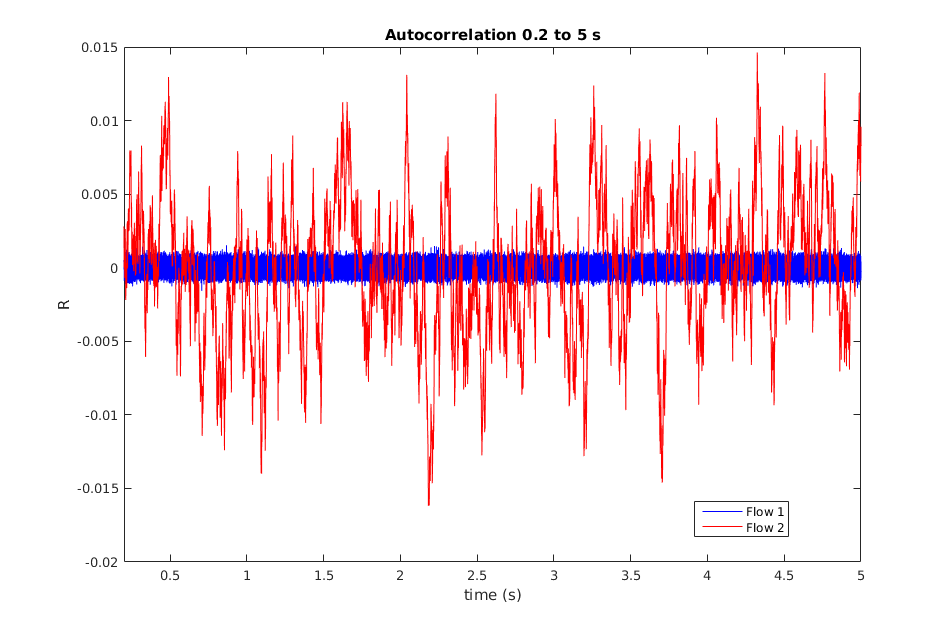
\includegraphics[scale=0.5]{./TEXT/auto2.png}
\caption{The comparison between the autocorrelation behaviours of the two flows between $0.2$ and $5$ s.}
\label{auto2}
\end{figure}